\chapter[Implementación]{Implementación}
\label{Chap5}

\section{Creación de Spiders}
Una vez instalado Scrapy, en el directorio escogido se usa el siguiente comando para generar un nuevo proyecto de Scrapy.

\begin{lstlisting}
	scrapy startproject miproyecto
\end{lstlisting}

El cual crea un nuevo directorio con el siguiente contenido.

\begin{figure} [h!]
	\centering
	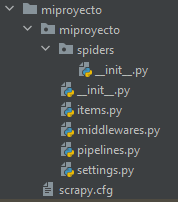
\includegraphics[width=0.3\textwidth]{fig/estructura_proyecto_scrapy.png}
	\caption[Estructura del proyecto recién creado]{Estructura del proyecto recién creado}
	\label{fig:ej11}
\end{figure}

En el directorio recientemente creado, se ejecuta el comando encargado de crear la Spider.

\begin{lstlisting}
	cd miproyecto
	scrapy genspider mispider webausar.com
\end{lstlisting}

En caso de no especificar el protocolo usado por la web, Scrapy asumirá que usa HTTPS.\newline
\newline
Tras ejecutar el comando la Spider habrá sido generada dentro de la carpeta spiders.

\begin{figure} [h!]
	\centering
	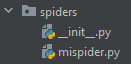
\includegraphics[width=0.2\textwidth]{fig/primera_spider.png}
	\caption[Directorio de almacenamiento de las Spider]{Directorio de almacenamiento de las Spider}
	\label{fig:ej12}
\end{figure}

Una vez abierto el archivo dispone del siguiente código.

\begin{lstlisting}[language=Python, caption={Spider recién generada}]
	import scrapy
	
	
	class MispiderSpider(scrapy.Spider):
		name = "mispider"
		allowed_domains = ["webausar.com"]
		start_urls = ["https://webausar.com"]
	
		def parse(self, response):
			pass
\end{lstlisting}

Scrapy usa una programación orientada a objetos, siendo cada Spider una clase representada dentro del proyecto.\newline
\newline
Analizando las variables definidas vemos las siguientes, \textit{name}, nombre por el que referenciar la Spider a la hora de ejecutarla; \textit{allowed\_domains}, indica que dominios está permitido visitar, es importante no especificar protocolo, de esta manera funcionara para cualquier web ya sea HTTP como HTTPS que pertenezca a ese dominio, de lo contrario se limitara al protocolo indicado; \textit{start\_urls}, URL inicial sobre la que se hará la request de petición de datos.\newline
\newline
El método \textit{parse()} es aquel al que se envía la respuesta obtenida de la web, para realizar el filtrado de la información deseada. Este método es invocado automáticamente por la Spider, sin necesidad real de hacerlo manualmente. Puede ser un método recursivo en caso de así quererlo o incluso se pueden definir nuevas funciones \textit{parse()} (usando un nombre distinto) en caso de necesitarlas.

\subsection{Proceso de obtención de datos}
Para poder realizar es la extracción de los datos, primero se debe ir a la web deseada e inspeccionar su estructuración HTML. Para ello, como ejemplo, se va a usar la web de Aemet.\newline

\begin{figure} [H]
	\centering
	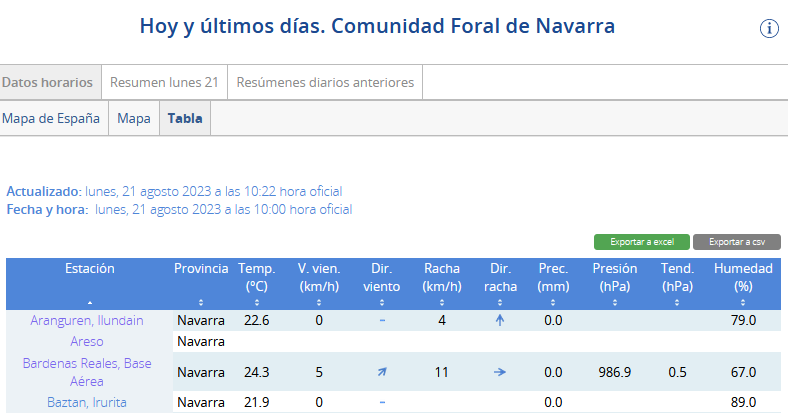
\includegraphics[width=0.8\textwidth]{fig/AemetCode.png}
	\caption[URL de inicio para obtener los códigos de las estaciones de Aemet]{Web de Aemet para obtención de datos}
	\label{fig:ej13}
\end{figure}

Accediendo mediante el F12 a la herramienta de inspección, se busca el elemento representativo de los datos deseados. En este caso, el nombre y código de la estación. Ambos se encuentran en el mismo elemento que forma la primera columna de la tabla.\newline

\begin{lstlisting}[caption={Estructura HTML de los datos deseados Aemet}]
	<table id="table">
		<thead></thead>
		<tbody>
			<tr class="fila_par">
				<td>
					<a href="/es/eltiempo/observacion/ultimosdatos?k=nav&"
					"amp;l=9263X&amp;w=0&amp;datos=det&"
					"amp;f=precipitacion">Aranguren, Ilundain</a>
				</td>
				...
			</tr>
			...
		</tbody>
	</table>
\end{lstlisting}

En este caso es posible filtrar fácilmente los datos, obteniendo todos directamente, aunque lo más común sería obtener las filas primero para luego iterar por cada una de ellas. Para obtenerlos se puede hacer mediante el selector de XPath como con el de CSS.\newline
\newline
Ambos se pueden obtener fácilmente en la herramienta de inspección, una vez seleccionado el elemento deseado, click derecho sobre el y, en el apartado copiar se mostrará la posibilidad de copiar ambos selectores. Es probable que el selector proporcionado no sea del todo lo que se busque o se pueda simplificar, por lo que es recomendable comprobarlo manualmente.\newline

\begin{lstlisting}
	rows = response.xpath('//div[@id="contenedor_tabla"]/table/tbody/tr/td/a')
	
	rows = response.css("div#contenedor_tabla tbody tr a")
\end{lstlisting}

Esto devuelve una lista de objetos tipo Selector, cosa que permite conforme se itera por cada elemento, volver a usar un selector para filtrar unicamente los datos deseados. En este caso.

\begin{lstlisting}
	path = rows[i].xpath("@href").get()
	name = rows[i].xpath("./text()").get()
	
	path = rows[i].css("*::attr(href)").get()
	name = rows[i].css("*::text").get()
\end{lstlisting}

De esta forma, mediante el uso de la función \textit{get()}, se pasa de tener un objeto Selector a un String. El uso de \textit{get()} sobre una lista devuelve el primer elemento, en caso de querer transformar toda la lista el método a usar es \textit{getall()}.\newline
\newline
Finalmente, como de la URL obtenida,
\begin{verbatim}
	('/es/eltiempo/observacion/ultimosdatos?k=nav&l=9263X&w=0&datos=det&f=precipitacion')
\end{verbatim}
solo es de interés el código de la estación (parámetro l de la query empezando por 0), se filtra mediante \textit{split()}.

\begin{lstlisting}
	code = path.split('&')[1].split('=')[1]
\end{lstlisting}

\subsection{Guardado de datos}
Scrapy almacena los datos en forma de múltiples diccionarios, tantos como webs usadas. Para acceder a esta información Scrapy proporciona dos alternativas, el uso de Items junto a ItemLoaders, siendo clases especificas de Scrapy o, mediante la palabra reservada \textit{yield} de Python, que tiene una funcionalidad parecida a \textit{return}, siendo esta la opción elegida debido a su fácil implementación.

\begin{lstlisting}[language=Python, caption={Guardar datos}]
	yield {
		'estacion': name,
		'codigo': path.split('&')[1].split('=')[1],
	}
\end{lstlisting}

Actualmente, si se ejecuta la Spider imprimirá los datos obtenidos por pantalla, aunque pueden ser almacenados en un fichero tanto CSV como JSON, a la hora de ejecutar la Spider añadiendo en el comando \textit{-o nombre.csv} ó \textit{-o nombre.json}.\newline
\newline
Para un uso ligero de forma manual, esa alternativa es más que suficiente, pero en este proyecto, al querer ejecutarlas de forma automática mediante el uso de Runners, se debe se implementar una variable llamada \textit{custom\_settings} para cada una de las Spider. Esta permite, sin la necesidad de modificar el archivo settings.py, añadir configuraciones o dependencias independientes en las Spiders.

\begin{lstlisting}[language=Python, caption={Confugurar guardado en JSON}]
	custom_settings = {
		'FEEDS': {
			'JSONs/RawCode/codigos_aemet.json': {
				'format': 'json',
				'encoding': 'utf-8',
				'overwrite': True,
			}
		}
	}
\end{lstlisting}

Indicando que, en la ruta que se especifica, almacene un fichero JSON utf-8 y, que cada vez que se llame a esta Spider sobre-escriba el fichero anterior.

\subsection{Spider básica}
Tras realizar los pasos, esta es la Spider básica terminada.

\begin{lstlisting}[language=Python, caption={Spider de ejemplo (Aemet Code Spider)}]
	import scrapy
	
	
	class AemetCodeSpider(scrapy.Spider):
		name = "aemet_code"
		allowed_domains = ["www.aemet.es"]
		start_urls = ["https://www.aemet.es/es/eltiempo/observacion/"
		"ultimosdatos?k=nav&w=0&datos=det&x=h24&f=precipitacion"]
		custom_settings = {
			'FEEDS': {
				'JSONs/RawCode/codigos_aemet.json': {
					'format': 'json',
					'encoding': 'utf-8',
					'overwrite': True,
				}
			}
		}
	
		def parse(self, response):
			rows = response.css("div#contenedor_tabla tbody tr a")
			
			for row in rows:
				path = row.xpath("@href").get()
				name = row.xpath("./text()").get()
				code = path.split('&')[1].split('=')[1]
			
			yield {
				'estacion': name,
				'codigo': code,
			}
\end{lstlisting}

\subsection{Método \textit{start\_requests()}}
El método \textit{start\_requests()} es llamado de forma automática al iniciar la Spider, siendo el encargado de hacer la llamada a la web indicada en \textit{start\_urls} y, una vez obtenidos los datos llamar a la función \textit{parse()}. Todo mediante un objeto Request de Scrapy, el cual devolverá un objeto tipo HTMLResponse. En caso de querer alterar el funcionamiento de la Spider este es el método a sobre-escribir.\newline
\newline
Como se quiere obtener los datos de todas las estaciones dentro de un mismo dominio, se sobre-escribe la función para recorrer el JSON con los códigos de estas y, hacer una llamada por estación con Request.\newline
\newline
El código quedaría de la siguiente manera.

\begin{lstlisting}[language=Python, caption={Sobre-escritura de \textit{start\_requests()}}]
	import json
	
	
	def start_requests(self):
		with open("JSONs/RawCode/codigos_aemet.json", encoding="utf-8") as f:
			data = json.load(f)
		for estacion in data:
			url = f'https://www.aemet.es/es/eltiempo/observacion'
			'/ultimosdatos?k=nav&l={estacion["codigo"]}&w=0&'
			'datos=det&x=&f=temperatura'
			yield scrapy.Request(url, self.parse)
\end{lstlisting}

Al definir la función de esta manera, no es necesario declarar la variable \textit{start\_urls}, por lo que siempre que se necesite sobre-escribir la función, no se usará la variable.

\subsection{Eliminar Log}
Cuando se verifique el correcto funcionamiento de la Spider, es recomendable quitar el máximo numero de Log por pantalla posible, es por eso que, en el fichero settings.py se escribirán las siguientes lineas.

\begin{lstlisting}[language=Python, caption={Configurar LOG}]
	LOG_LEVEL = 'WARNING'
	LOG_ENABLED = False
\end{lstlisting}

\section{Spiders usadas}
Para este proyecto se han creado cuatro proyectos de Scrapy, uno por cada web.

\subsection{Aemet}
Siendo la Spider de obtención de códigos la usada como ejemplo, no hay mucho más que comentar al respecto de ella, obtiene los nombres y códigos de cada estación.

\subsubsection{Data Spider}
La Spider de obtención de datos es un poco más compleja, necesitando sobre-escribir la función de \textit{start\_requests()} como se muestra en el ejemplo del apartado anterior. Primero lee el fichero JSON con los códigos de las estaciones, itera por ellos y, crea una llamada Request por cada estación.

Dentro de la función \textit{parse()}:

\begin{lstlisting}[language=Python, caption={Selector en \textit{parse()} de Aemet Data Spider}]
	latitud = response.css('abbr.latitude::text').get()
	longitud = response.css('abbr.longitude::text').get()
	estacion = response.css("a.separador_pestanhas").get()
	rows = response.css('tbody tr')
\end{lstlisting}

Obtiene las coordenadas, latitud, longitud; una URL con el código de la estación, variable estacion y, todas las filas presentes en el cuerpo de la tabla de datos, rows.

\begin{lstlisting}[language=Python, caption={Trabajar sobre los datos de Aemet Data Spider}]
	datos = []
	for row in rows:
		dato = {
			'fecha y hora': row.xpath('./td[1]/text()').get() + ':00',
			'temperatura (C)': row.xpath('./td[2]/text()').get(),
			'humedad (%)': row.xpath('./td[10]/text()').get(),
			'precipitacion (mm)': row.xpath('./td[7]/text()').get(),
		}
		
		if dato['precipitacion (mm)'] != " ":
			datos.append(dato)
\end{lstlisting}

Se crea una lista datos vacía para almacenar los datos. Posteriormente, se recorren las filas obtenidas, creando un objeto JSON llamado dato, que almacena, obteniendo mediante selectores, la fecha y hora (añadiendo :00 al final para tener el mismo formato dd/mm/aa hh:mm:ss que en el resto de webs), la temperatura, la humedad y la precipitación.\newline
\newline
En caso de que el apartado precipitación no esté vació, pues puede darse el caso en el que la web aun no disponga de el a cierta hora, pero si muestre esta franja horaria pues dispone de otros datos como pueden ser aquellos relacionados con el viento, el objeto dato sera almacenado en la lista datos.

\begin{lstlisting}[language=Python, caption={Guardado de datos de Aemet Data Spider}]
	yield {
		'coordenadas': latitud + ' | ' + longitud,
		'estacion': estacion.split('=')[3].split('&')[0],
		'datos': datos,
	}
\end{lstlisting}

Finalmente se almacenan las coordenadas con un formato global para todas las plataformas y, se filtra mediante splits el código de la estación.

\subsection{CHCantábrico}

\subsubsection{Code Spider}
La Spider para la adquisición de códigos de CHCantábrico no necesita de sobre-escritura del método \textit{start\_requests()}, por lo que el código a analizar sera el presente en la función \textit{parse()}.

\begin{lstlisting}[language=Python, caption={Selector en \textit{parse()} de CHCantábrico Code Spider}]
	rows = response.xpath('//table[@class="tablefixedheader niveles"]/tbody/tr')
\end{lstlisting}

Puesto que la estructuración HTML de la web no proporciona una manera clara de lograr los datos mediante un selector CSS, los datos se logran filtrar por su selector XPath. De este, se obtendrán las filas que representan cada estación.

\begin{lstlisting}[language=Python, caption={Trabajar sobre los datos de CHCantábrico Code Spider}]
	for row in rows:
		codigoBusqueda = row.css('td.codigo::text').get()
		limites = row.css('table.umbrales_gr td.datos::text').getall()
		path = row.xpath('./td/a/@href').getall()[-1]
		estacion = row.xpath('./td/a/text()').getall()[-3]
\end{lstlisting}

Una vez obtenidas las filas, se itera sobre ellas para obtener, dos códigos, el primero, codigoBusqueda como código representativo de la estación cara a obtener las coordenadas y, el código necesario para acceder a los datos, inicialmente almacenado en una URL en la variable path; los limites marcados de pre-alerta, alerta y seguimiento en la variable limites, siendo estos una buena base para empezar con las predicciones de inundación y, el nombre de la estación.\newline
\newline
Inicialmente, para las variables path y estacion, se obtienen todo los elementos que corresponden con el selector asignado, para posteriormente quedarse con el que realmente interesa. Se hace así al no poder filtrar mediante HTML los datos concretos.

\begin{lstlisting}[language=Python, caption={Combrobar limites de CHCantábrico Code Spider}]
	for i in range(len(limites)):
		if limites[i] == 'No definido':
			limites[i] = None
\end{lstlisting}

Aun dentro del bucle, se comprueba si los limites están definidos, marcando como None (null) aquellos que no lo estén.

\begin{lstlisting}[language=Python, caption={Guardado de datos de CHCantábrico Code Spider}]
	yield {
		'estacion': estacion,
		'codigo': path.split("=")[-1],
		'codigoSecundario': codigoBusqueda,
		'seguimiento': limites[0],
		'prealerta': limites[1],
		'alerta': limites[2],
	}
\end{lstlisting}

Por ultimo, se filtra el código de la estación (aquel usado para acceder los datos) de la URL y, se guardan los datos.

\subsubsection{Data Spiders}
CHCantábrico muestra datos tanto del nivel del río como de la precipitación, aunque lo hace en dos direcciones distintas, haciendo necesario el uso de dos Spiders.\newline
\newline
Puesto que ambas comparten la misma estructuración de código, solo se explicara una de ellas. La de nivel del río.

\begin{lstlisting}[language=Python, caption={Función \textit{start\_requests()} CHCantábrico Nivel Spider}]
	def start_requests(self):
		with open("JSONs/RawCode/codigos_chcantabrico.json", encoding="utf-8") as f:
			data = json.load(f)
		for estacion in data:
			params_nivel = {
				'p_p_id': 'GraficaEstacion_INSTANCE_wH0LL6jTUysu',
				'p_p_lifecycle': '2',
				'p_p_state': 'normal',
				'p_p_mode': 'view',
				'p_p_resource_id': 'downloadCsv',
				'p_p_cacheability': 'cacheLevelPage',
				'_GraficaEstacion_INSTANCE_wH0LL6jTUysu_cod_estacion': f'{estacion["codigo"]}',
				'_GraficaEstacion_INSTANCE_wH0LL6jTUysu_tipodato': 'nivel',
			}
		
			url = 'https://www.chcantabrico.es/evolucion-de-niveles'
			
			yield scrapy.FormRequest(url=url,
				method='GET',
				formdata=params_nivel,
				callback=self.parse,
				cb_kwargs={'estacion': estacion['codigo']}
			)
\end{lstlisting}

Como se necesitan los datos de todas las estaciones, se reescribirá la función \textit{start\_requests()}.\newline
\newline
A su vez, como CHCantábrico no muestra los datos por pantalla, incluyendo un botón sobre el que pulsar para obtenerlos descargando un fichero CSV, en vez de hacer una request básica mediante la clase Request, se hace uso uso de FormRequest para hacer una llamada GET, que simular la llamada a un formulario y obtiene los datos que este devuelve.\newline
\newline
De esta forma, pasandole los parámetros necesarios en el argumento formdata a la URL indicada, definidos como un diccionario en la variable params\_nivel, se obtendrán los datos sin la necesidad de ningún CSV. simulando en cierto modo una llamada mediante cURL.\newline
\newline
Cabe mencionar que, Request devuelve un HTMLResponse y que, la respuesta de estas llamadas no es código HTML, por lo que, aun en caso de que llegue a ser posible usar Request, es más correcto el uso de FormRequest devolviendo un FormResponse para este tipo de casos.\newline
\newline
El uso del argumento cb\_kwargs sirve para enviar un mayor numero de argumentos a la función \textit{parse()} de los que normalmente recibe.

\begin{lstlisting}[language=Python, caption={Función \textit{parse()} CHCantábrico Nivel Spider}]
	def parse(self, response, estacion):
		if not response.text.startswith('-'):
			urlData = response.text
			rawData = pd.read_csv(io.StringIO(urlData), delimiter=';', encoding='utf-8', header=1)
			rawData.columns = ['fecha y hora', 'nivel (m)']
			parsedData = rawData.to_json(orient="records")
\end{lstlisting}

Debido al argumento cb\_kwargs, la función \textit{parse()} recibe un tercer argumento, estación. En este caso, para poder enviar a cada conjunto de datos recibidos el código de la estación a la que pertenecen, pues dentro de la respuesta obtenida solo se proporciona el nombre de esta.\newline
\newline
Dentro de la función \textit{parse()} lo primero que se hace es comprobar que realmente se ha recibido una respuesta correcta, pues, aunque todas la estaciones disponen de datos del nivel del río, no todas disponen los de precipitación. El problema viene cuando a estas estaciones se les piden los datos, ya que en vez de enviar un error 404 como seria esperado.

\begin{verbatim}
	-
	FECHA;VALOR(mm)
\end{verbatim}

Una alternativa para deshacerse de esta comprobación sería eliminar aquellas estaciones que no proporcionen datos o filtrandolas para no hacer la llamada directamente, aunque esto no solo resultaría más complejo, si no que crearía el problema de que cada cierto tiempo habría que comprobar si alguna estación ha empezado a proporcionar datos para incluirla nuevamente en la lista de estaciones a las cuales hacer llamada.\newline
\newline
Una vez hecha la comprobación, en caso de que no sea una respuesta vacía, el texto viene proporcionado con el siguiente formato.

\begin{verbatim}
	Ribera de Piquín
	FECHA;VALOR(m)
	03/08/2023 11:30:00;0.153
	03/08/2023 11:45:00;0.153
	03/08/2023 12:00:00;0.153
	...
\end{verbatim}

Al tener formato CSV se lee mediante la función read\_csv() incluida en la librería pandas, se indica el delimitador, la codificación y la linea que representa la cabecera, empezando de la 0, en este caso la 1, pues no nos interesa el nombre de la estación. Finalmente, como la función espera que se le pase una ruta a un fichero, lo que hacemos mediante io.StringIO() es crear un objeto con el que simular un fichero en memoria, pasando de disponer texto plano a un DataFrame de pandas.\newline
\newline
Como últimos pasos, se cambian los nombres de las cabeceras a aquellos definidos de forma global para todas las webs y, se convierte el DataFrame en un JSON con la función to\_json() indicando que el formato sea "records", esto implica que cada linea del DataFrame va a representar un objeto JSON.

\begin{lstlisting}[language=Python, caption={Guardado de datos de CHCantábrico Nivel Spider}]
	yield {
		'estacion': estacion,
		'datos': json.loads(parsedData)
	}
\end{lstlisting}

Con el uso de la función loads() de la librería json nos aseguramos el correcto formato del JSON.

\subsubsection{Coordenates Spider}
Aunque en la web misma de CHCantárico se proporciona un mapa indicando la localización de cada estación, las coordenadas de esta no están disponibles para adquirir dentro de la web, es por eso que es necesario el uso de la web del centro de estudios hidrológicos para poder obtener las coordenadas.\newline
\newline
En esta página se pueden encontrar mediante el "codigoSecundario" anteriormente obtenido, desgraciadamente, no todas las estaciones incluidas en CHCantábrico están listadas en esta página, siendo el mayor inconveniente para el correcto funcionamiento del apartado de predicción.

\begin{lstlisting}[language=Python, caption={Selector en \textit{parse()} de CHCantábrico Coordinates Spider}]
	longitud = response.css('p::text')[6].get().strip()
	latitud = response.css('p::text')[7].get().strip()
	estacion = response.css('font::text')[14].get().strip()
\end{lstlisting}

\begin{lstlisting}[language=Python, caption={Guardado de datos de CHCantábrico Coordinates Spider}]
	yield {
		'coordenadas': f'Lat: {latitud} | Lon: {longitud}',
		'estacion': estacion,
	}
\end{lstlisting}

Exceptuando el uso del "codigoSecundario" para referenciar estaciones, esta es una Spider muy simple la cual no dispone de nada que no haya sido anteriormente explicado.

\subsubsection{Código descartado}
Siendo CHCantábrico la primera web de la que se obtuvo los datos, sin gran conocimiento de Scrapy y sobre todo, sin saber realmente como sería la plataforma, el planteamiento de la obtención de datos se realizo de forma ajena a las Spider de Scrapy.\newline
\newline
Viendo que los datos no están presentes en la web y, que Scrapy no dispone de interacción JavaScript por defecto, la única alternativa viable conocida en esos momentos fue probar a realizar una llamada cURL por terminal, al ver que efectivamente mediante cURL era posible obtener los datos deseados, se escribió un script para los datos de nivel y otro para los de precipitación.

\begin{lstlisting}[language=Python, caption={Script de obtención de datos pluviometricos descartado}]
	import pandas as pd
	import io
	import requests
	import json
	
	with open('codigos_estaciones_chcantabrico.json', 'r', encoding='utf-8') as f:
		data = json.load(f)
		
	datos = []
	for item in data:
		params_pluvio = {
			'p_p_id': 'GraficaEstacion_INSTANCE_ND81Xo17PIZ7',
			'p_p_lifecycle': '2',
			'p_p_state': 'normal',
			'p_p_mode': 'view',
			'p_p_resource_id': 'downloadCsvPluvio',
			'p_p_cacheability': 'cacheLevelPage',
			'_GraficaEstacion_INSTANCE_ND81Xo17PIZ7_cod_estacion': f'{item["codigo"]}',
			'_GraficaEstacion_INSTANCE_ND81Xo17PIZ7_tipodato': 'pluvio',
		}
		
		response_pluvio = requests.get('https://www.chcantabrico.es/precipitacion-acumulada', params=params_pluvio)
		if response_pluvio.status_code == 200:
			if not response_pluvio.text.startswith('-'):
				urlData = response_pluvio.text
				rawData = pd.read_csv(io.StringIO(urlData), delimiter=';', encoding='utf-8', header=1)
				rawData.columns = ['fecha y hora', 'precipitacion (mm)']
				parsedData = rawData.to_json(orient="records")
				
				estacion = {
					'estacion': item["codigo"],
					'datos': json.loads(parsedData)
				}
				datos.append(estacion)
			else:
				print(f'{item["estacion"]} Error retrieving data: 404')
				print("-------------------")
		else:
			print(f'{item["estacion"]} Error retrieving data: {response_pluvio.status_code}')
			print("-------------------")
	
	with open('../../JSONs/RawData/datos_pluvio_chcantabrico.json', 'w', encoding='utf-8') as outfile:
		json.dump(datos, outfile)
\end{lstlisting}

Todo el apartado de tratamiento de los datos es prácticamente idéntico al realizado con la Spider, solo que en vez de usar FormRequest, se hace uso de la librería requests para realizar la llamada \textit{get()}, tras realizarla, se comprueba que haya sido exitosa (esta comprobación la realiza Scrapy automáticamente) y, en caso de serlo se realiza todo el tratamiento, guardando los datos en la lista datos. Una vez realizadas todas las llamadas, guardamos los datos obtenidos usando la función json.dump().\newline
\newline
Aunque en esta versión se almacenan todos los datos en un mismo JSON, originalmente los datos eran guardados en un CSV por cada estación, de tal manera que el nombre del CSV era el mismo que el de la estación perteneciente. Más adelante al consolidar más la plataforma, sobre todo el uso de Django para la creación de una API, se vio que era más útil guardar los datos no solo en formato JSON si no disponer de un único fichero por estación, de esta forma solo seria necesario realizar una única llamada por estación a la API para cargar los datos. Llegando a esta versión del script.\newline
\newline
Posteriormente, llegado el momento de la automatización quedo claro que, aun siendo posible automatizar el proceso con el script anterior, iba a suponer un problema para la modularidad del proyecto. Pues tener múltiples scripts de diferentes fuentes, solo aumentaba la complejidad a la hora de crear un script ya sea en Python o Bash encargado de ejecutar cada parte individual de cada web. Siendo la alternativa proporcionada por Scrapy de ejecutar múltiples Spider mediante un simple script Python la mejor opción.\newline
\newline
Es por eso que se investigo la posibilidad de obtener los datos mediante Scrapy, estudiando los diferentes objetos Request proporcionados, hasta llegar a la versión actual con el uso de FormRequest.

\subsection{MeteoNavarra}

\subsubsection{Code Spider}
La estructuración HTML de la web y la falta de experiencia son el motivo principal asociado a la complejidad de esta Spider, la mayor parte del tiempo a la hora de crearla ha sido invertido explorando el código HTML buscando la forma más optima de lograr los datos necesarios. Son múltiples las iteraciones sufridas hasta llegar a la versión actual.

\begin{lstlisting}[language=Python, caption={Selector en \textit{parse()} de MeteoNavarra Code Spider}]
	rows = response.css('div#tabAUTO script::text').getall()
\end{lstlisting}

Del selector se obtiene el código JavaScript perteneciente a cada fila de la tabla, siendo la forma mas sencilla de lograr tanto el nombre como el código de la estación.

\begin{lstlisting}[language=Python, caption={Guardado de datos de MeteoNavarra Code Spider}]	
	for row in rows:
		yield {
			'estacion': row.split(',')[3],
			'codigo': row.split(',')[0].split('(')[1],
		}
\end{lstlisting}

A la hora de guardar los datos, se itera por filas y se filtra del código aquellos deseados.

\subsubsection{Data Spider}
La necesidad de recorrer múltiples estaciones, obliga como en el resto de Spiders de obtención de datos, a sobre escribir la función \textit{start\_requests()}.

\begin{lstlisting}[language=Python, caption={Uso de fechas en función \textit{start\_requests()} MeteoNavarra Data Spider}]
	import datetime

	current_date = datetime.date.today()
	delta = datetime.timedelta(days=1)
	tomorrow_date = current_date + delta
	yesterday_date = current_date - delta
	tomorrow_date_format = tomorrow_date.strftime(" %d%%2F %m%%2F%Y").replace(' 0', '')
	yesterday_date_format = yesterday_date.strftime(" %d%%2F %m%%2F%Y").replace(' 0', '')
\end{lstlisting}

La curiosidad en esta radica en que, a diferencia del resto de páginas, que definen automáticamente una franja de fechas a mostrar, meteoNavarra fuerza la necesidad de que el usuario elija las fechas que desee ver, es por eso que hace uso de la librería datetime, pues facilita el trabajo con fechas.\newline
\newline
Con la intención de que funcione proporcionando fechas distintas cada día se realiza el siguiente proceso. Se obtiene la fecha actual con la función today(), con el método timedelta(days=1) se crea un objeto timedelta que representa una duración de un día, gracia a el, se calcula el día de mañana y el de ayer, sumando y restando esa duración al día de hoy. Para terminar, puesto que la fecha debe ir incluida en una URL, mediante el método strftime(), formateamos los datetime calculados para que correspondan con el codificado URL.\newline
\newline

\begin{lstlisting}[language=Python, caption={Selector en \textit{parse()} de MeteoNavarra Data Spider}]
	rows = response.css('table.border tr:not([bgcolor*="#FFFFFF"])')
	estacion = response.css('table a::attr(href)')[7].get()
\end{lstlisting}

De los siguientes selectores cabe mencionar el primero. Aunque en la web se hace uso del elemento HTML table, este no indica que elementos tr pertenecen a la cabecera o al cuerpo de la tabla con el uso de thead y tbody, por el contrario, las filas correspondientes a la cabecera se muestran con el color de fondo representado hexadecimalmente \#FFFFFF. Es por eso que se indica explícitamente no obtener esas filas con el uso de tr:not([bgcolor*="\#FFFFFF"]).

\begin{lstlisting}[language=Python, caption={Trabajar sobre los datos de MeteoNavarra Data Spider}]
	datos = []
	for row in rows:
		dato = {
			'fecha y hora': row.xpath('./td[1]/text()').get().strip().replace(' ', ' ') + ':00',
			'temperatura (C)': row.xpath('./td[2]/font/text()').get(),
			'humedad relativa (%)': row.xpath('./td[3]/font/text()').get(),
			'radiacion global (W/m^2)': row.xpath('./td[4]/font/text()').get(),
			'precipitacion (l/mm^2)': row.xpath('./td[5]/font/text()').get(),
		}
		
		if dato['radiacion global (W/m^2)'] == '- -':
			dato['radiacion global (W/m^2)'] = None
		
		if dato['precipitacion (l/mm^2)'] != '- -':
			datos.append(dato)
\end{lstlisting}

En la función \textit{parse()}, como en otras Spider, se crea una lista datos vacía que es llenada con los objetos JSON obtenidos al recorrer cada fila de las anteriormente obtenidas y, filtrar mediante selectores aquellos datos de utilidad.\newline
\newline
Luego, se comprueba la disponibilidad de un valor numérico de radiación global, pues en caso de no existir, la web proporciona '- -'. Posteriormente, puesto que la web muestra todas las franjas horarias dentro del que se corresponde con el día actual, se eliminan todas esas horas sin datos con la comprobación respecto a la precipitación.\newline
\newline

\begin{lstlisting}[language=Python, caption={Comprobacion exitencia de datos y guardado de MeteoNavarra Data Spider}]
	if datos:
		yield {
			'estacion': estacion.split('idestacion=')[1].split('&')[0],
			'datos': datos,
		}
\end{lstlisting}

A continuación, en caso de que existan datos a guardar, pues algunas de las estaciones puedes llegar a no disponer de datos, se realiza el \textit{yield}.

\begin{lstlisting}[language=Python, caption={Navegacion a segunda página de datos en MeteoNavarra Data Spider}]
	next_page = response.css("table a::attr(href)").getall()
	page_number = response.xpath("//b/text()").getall()
	if not page_number[0] == page_number[1]:
		next_page = response.urljoin(next_page[7])
		yield scrapy.Request(next_page, callback=self.parse)
\end{lstlisting}

Finalmente, aun dentro de \textit{parse()}, como los datos de ciertas estaciones están repartidos en dos páginas, adquiere la posible URL a la segunda página y, el numero de la página actual y siguiente, en caso de que los números sean distintos, navega a esa segunda página para realizar el mismo proceso descrito anteriormente.\newline
\newline
Esto es posible gracias a que \textit{yield}, aunque a groso modo funcione como un return, no fuerza el final de la ejecución, por lo que todo código por debajo de este sera ejecutado, llegando a haber múltiples \textit{yield} en una misma función.

\subsubsection{Coordenates Spider}
Por último, necesitamos de una Spider para la obtención de las coordenadas pues no están disponibles para obtener dentro de las páginas anteriores, aunque sí dentro del mismo dominio.\newline
\newline
Mediante \textit{start\_requests()}, realiza tantas llamadas como estaciones.

\begin{lstlisting}[language=Python, caption={Selector en \textit{parse()} de MeteoNavarra Coordenates Spider}]
	coordenadas = response.css('td::text')[19].get()
	estacion = response.css('input::attr(value)').get()
\end{lstlisting}

Una vez en la función \textit{parse()}, toma las coordenadas mostradas en una tabla y, obtiene el código de la estación del atributo value de un input.

\begin{lstlisting}[language=Python, caption={Guardado de datos de MeteoNavarra Coordenates Spider}]
	yield {
		'coordenadas': coordenadas.strip().replace('\r\n\t\t', ' ').replace(' (*)', ''),
		'estacion': estacion,
	}
\end{lstlisting}

Finalmente, las coordenadas, con el fin de verse bien en la web, en vez de estar estilizadas con CSS, vienen estilizadas con elementos textuales, los cuales son eliminados.

\subsection{Agua en Navarra}
Las Spiders de Agua en Navarra son las más complejas entre todas, usando una filosofía ligeramente distinta al resto de Spiders y, por el uso de Selemiun para poder interactuar con la web mediante JavaScipt.\newline
\newline
Ambas Spider, Code y Data, parten de las misma \textit{start\_urls} y van recorriendo las páginas presentes hasta llegar a aquella que muestre los datos deseados. Esto se debe hasta cierto punto a la estructuración de la página, haciendo más sencillo navegar por ella que crear una Spider por cada página a visitar. La navegación por la web se realiza usando múltiples funciones de la misma naturaleza que \textit{parse()}.\newline
\newline
Para Data Spider esto implica no necesitar de un fichero JSON del cual leer los códigos de las estaciones.\newline
\newline

\begin{lstlisting}[language=Python, caption={Función \textit{parse()} Agua en Navarra Spiders}]
	def parse(self, response):
		for link in response.css('dl#navarramap a::attr(href)'):
			if link.get() != 'ctaMapa.aspx?IdMapa=1&IDOrigenDatos=1':
				yield response.follow(link.get(), callback=self.parse_area)
\end{lstlisting}

La función \textit{parse()} es compartida por ambas Spider. Extrae los link representantes de cada área definida sobre el mapa y, navega por todos ellos a excepción del link de origen, aquel en el que se encuentra.\newline
\newline
El uso de \textit{response.follow()} es equivalente a realizar un Request, pero no necesita pararle una URL completa, solo con la ruta es capaz de generar la llamada, en caso de necesitar explícitamente el uso de Request esta seria la manera.

\begin{verbatim}
	yield Request(url=response.urljoin(link.get()), callback=self.parse_area)
\end{verbatim}

De ambas formas, en el argumento callback se indica a que función debe realizar la llamada, pasando de \textit{parse()} a \textit{parse\_area()}.

\begin{lstlisting}[language=Python, caption={Función \textit{parse\_area()} Agua en Navarra Spiders}]
	def parse_area(self, response):
		for link in response.css('area[shape="rect"]::attr(href)'):
			yield response.follow(link.get(), callback=self.parse_estacion)
\end{lstlisting}

Siendo la última función implementada de la misma manera en las Spider. Se realiza el mismo proceso, obtiene todos los link a las webs, ya sí, de la estación y, llama a \textit{parse\_estacion()}.

\subsubsection{Code Spider}

\begin{lstlisting}[language=Python, caption={Función \textit{parse\_estacion()} Agua en Navarra Code Spider}]
	def parse_estacion(self, response):
		urls = response.xpath('//span/a/@href').getall()
		estacion = response.css('div#bloq_iconos span span::text').getall()
		codigoEstacion = response.css("form#frmDatosEstacion::attr(action)").get()
		
		codigos = []
		for url in urls:
			codigos.append(url.split('=')[1])
\end{lstlisting}

Una vez en la función \textit{parse\_estacion()} de Code Spider, como ocurre con CHCantábrico, la estación dispone de múltiples códigos, aquel que referencia la estación, uno para el nivel y aunque no en todas, otro para el caudal del río.\newline
\newline
Tanto el código de nivel y caudal del río originalmente se almacenan en la variable urls, almacenando las direcciones en las cuales están presentes. Posteriormente, se toma de la URL y se guardan en la lista codigos.\newline
\newline
La variable estación es una lista que almacena, la descripción de la estación, el municipio al que pertenece, el río y, las coordenadas.

\begin{lstlisting}[language=Python, caption={Guardado de datos de Agua en Navarra Code Spider}]
	yield {
		'descripcion': estacion[0],
		'municipio': estacion[1],
		'rio': estacion[2],
		'coordenadas': estacion[3],
		'estacion': codigoEstacion.split('=')[-1],
		'codigos': codigos,
	}
\end{lstlisting}

Al final estos datos son almacenados.

\subsubsection{Data Spider}

\begin{lstlisting}[language=Python, caption={Función \textit{parse\_estacion()} Agua en Navarra Data Spider}]
	from scrapy_selenium import SeleniumRequest
	from selenium.webdriver.common.by import By
	from selenium.webdriver.support import expected_conditions as EC
	
	def parse_estacion(self, response):
		for link in response.css('div#divResultadosAforo a::attr(href)'):
			yield SeleniumRequest(
				url=response.urljoin(link.get()),
				wait_time=2,
				wait_until=EC.element_to_be_clickable((By.ID, 'btnDatosNumericos')),
				callback=self.parse_data,
				script='document.querySelector("#btnDatosNumericos").click()',
			)
\end{lstlisting}

Lo primero que llama la atención de esta Spider respecto al resto, es el uso de SeleniumRequest, este tipo de objeto Request pertenece a la librería scrapy\_selenium, siendo una alternativa sencilla de unificar las funcionalidades de Selenium en Scrapy, de esta forma, se lidia con la falta de integración de interacción con JavaScript en Scrapy.\newline
\newline
Tras realizar el mismo proceso que antes, la Spider llega a la función \textit{parse\_estacion()}, esta vez, en vez de obtener los datos de la estación, accedemos a los links que permiten mostrar los datos mediante SeleniumRequest y llama a la función \textit{parse\_data()}.\newline
\newline
Como el link proporcionado dirige a una página que muestra los datos en forma de gráfica y, para acceder a los datos numéricos es necesario pulsar un botón, SeleniumRequest se configura de tal forma que, espera a que este esté correctamente cargado con el argumento wait\_until, indicando que elemento deseas esperar a ser cargado; en caso de que no se cargue, es recomendable usar el argumento wait\_time, que usado junto al anterior, establece el tiempo antes de dar la llamada por errónea; si el botón se carga correctamente, en el argumento script indicamos que se debe pulsar sobre este, llevándonos finalmente a los datos numéricos.\newline
\newline

\begin{lstlisting}[language=Python, caption={Selector en \textit{parse\_data()} de Agua en Navarra Data Spider}]
	tipo = response.css('span#lblSenal::text').get()
	estacion = response.css('li#cabecera_nombreEstacion a::attr(href)').get()
	fechas = response.css('span.cont_fecha_gra::text').getall()
	valores = response.css('span.cont_valor_gra::text').getall()
\end{lstlisting}

En la función \textit{parse\_data()}, se obtienen los datos por columna en vez de fila, pues la web no hace un correcto uso formateo por tabla, pues no existe esta tabla, insertando los datos sobre un elemento div y formateandolos posteriormente con CSS. Esta forma de mostrar los datos fuerza tener que obtener las fechas por un lado y los valores por otro, resultando en dos listas que debemos unir. La variable tipo (Nivel o caudal) es necesaria para posteriormente guardar los datos de forma correcta.

\begin{lstlisting}[language=Python, caption={Selector en \textit{parse\_data()} de Agua en Navarra Data Spider}]
	datos = []
	if tipo == "Nivel Rio":
		for i, fecha in enumerate(fechas):
			dato = {
				'fecha y hora': fecha.strip() + ':00',
				'nivel (m)': valores[i].strip(),
			}
			datos.append(dato)
	else:
		for i, fecha in enumerate(fechas):
			dato = {
				'fecha y hora': fecha.strip() + ':00',
				'caudal (m^3/s)': valores[i].strip(),
			}
			datos.append(dato)
	
	yield {
		'estacion': estacion.split('=')[-1],
		'datos': datos,
	}
\end{lstlisting}

Al hacer uso de una Spider para obtener todos los datos, estando presentes en distintas páginas, hace necesaria la comprobación inicial con la variable tipo de que datos estamos recibiendo, para poder almacenarlos correctamente. Una vez realizada, se itera la lista de fechas y se unen con su respectivo valor (el orden de los valores corresponde con el de las fechas) y se insertan el la lista datos. Finalmente son guardados.

\subsubsection{Configuración Selenium}
Para que Selenium funcione, es necesario incluir las siguientes lineas de código en el archivo settings.py generado por Scrapy.

\begin{lstlisting}[language=Python, caption={Agua en Navarra configuración Selenium}]
	from shutil import which
	
	SELENIUM_DRIVER_NAME = 'chrome'
	SELENIUM_DRIVER_EXECUTABLE_PATH = which('chromedriver')
	SELENIUM_DRIVER_ARGUMENTS = ['--headless',
	'--disable-logging',
	'--disable-in-process-stack-traces',
	'--log-level=1',
	'--disable-extensions'
	]
	
	DOWNLOADER_MIDDLEWARES = {
		'scrapy_selenium.SeleniumMiddleware': 800
	}
\end{lstlisting}

En este caso se indica que el navegador deseado para realizar el trabajo es Chrome y mediante el método which selecciona la ruta del ejecutable del driver de chrome.\newline
\newline
Los argumentos usados indican, --headless significa que las instancias de Chrome creadas sean sin interfaz, de esta forma no tendremos cientos de ventanas de Chrome abriéndose y cerrándose cada vez que se ejecute la Spider; --disable-logging como su nombre indica elimina el Log; --disable-in-process-stack-traces desactiva el stack-trace, esto se realiza unicamente con el fin de intentar mejorar el rendimiento; --log-level indica el tipo de log que se desea mostrar, siendo INFO = 0, ALERTA = 1, ERROR = 2 y FATAL = 3, aunque el Log este desactivado esta bien indicar que clase de Log deseas que aparezca en caso de que se vuelva a activar; --disable-extensions desactiva todas las extensiones que podamos tener instaladas, nuevamente con el fin de mejorar el rendimiento.\newline
\newline
Una vez incluido el middleware, ya solo quedaría descargar el driver de chrome.\newline
\newline
Chromedriver.exe puede ser obtenido en la web \url{https://chromedriver.chromium.org/downloads}, descargando aquel que corresponda a la versión de Chrome instalada. Una vez descomprimido debe ser incluido dentro de la carpeta de proyecto de Scrapy.

\begin{figure} [h!]
	\centering
	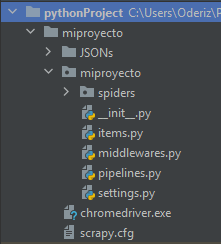
\includegraphics[width=0.4\textwidth]{fig/chromedriver.png}
	\caption[Ruta chromedriver.exe]{Ruta chromedriver.exe}
	\label{fig:ej15}
\end{figure}

En caso de estar en Windows con esto ya es suficiente, aunque al usar Debian son necesarios unos paso más para configurar chromedriver.

\begin{lstlisting}[caption={Configuración chromedriver Debian}]
	#Otorgamos permiso de ejecucion a chromedriver
	sudo chmod +x chromedriver
	
	#Movemos el .exe a directorio /usr/local/share/
	sudo mv chromedriver /usr/local/share/chromedriver
	
	#Creamos la relacion entre el .exe y el directorio
	sudo ln -s /usr/local/share/chromedriver /usr/bin/chromedriver
	
	#Ejecutamos
	chromedriver --version
	
	#En caso de haber realizado correctamente el proceso deberia aparecer
	una linea parecida a esta
	ChromeDriver 115.0.5790.110
	(5e87dfef0c85687ea835e444d33466745cc0725f-refs/branch-heads/5790_90@{#20})
\end{lstlisting}

Hecho esto ya estaría configurado chromedriver.

\subsubsection{Alternativas probadas}
Antes de saber que es necesario dirigirse a la pagina donde se muestra la gráfica para poder acceder a la página con los datos numéricos, se probo con una Spider que accedía directamente a esta. Visto que el resultado obtenido estaba vacío y, que en apariencia la Spider era correcta, obteniendo teóricamente aquellos datos deseados, se comprobó la web manualmente, resultando en la obtención del error mostrado en la figura \ref{fig:ej5}.\newline
\newline
Es por eso que, partiendo de un uso de Scrapy sin uso de extensiones de terceros, se probó una solución al problema que seguía la metodología de recorrer las webs, de esta manera, se visita inicialmente la web con la gráfica para posteriormente redirigirse a los datos numéricos. Resultando en un nuevo fracaso.\newline
\newline
Esta vez si que se obtenían datos, aunque no de forma correcta, muchas estaciones aparecían repetidas múltiples veces, de tres a siete veces en el peor de los casos visto. Siendo el resultado esperado la aparición de una misma estación un total de dos veces, una con los datos del caudal y otra por los datos del nivel. Tras volver a la comprobación manual, resulto en el mismo comportamiento, por alguna razón, una vez dentro de la web de los datos numéricos, al cambiar el código de la estación y recargar la pagina, lo mismo se actualizaban los datos para mostrar los de la nueva estación como no lo hacían, mostrando los datos de la anterior.\newline
\newline
Esto causó la incertidumbre de si era posible obtener datos la web de forma fiable. Finalmente, tras barajar la posibilidad de pulsar el botón para acceder los datos, se dio con la herramienta usada en la versión final, Selenium y, tiempo después con una alternativa más moderna a esta, Playwright.\newline
\newline
Por suerte, Selenium, al ser usado mediante la extensión scrapy\_selenium, resultó funcionar a la primera, aunque a un costo temporal relativamente alto, en comparación con las demás Spider, con una media de dos minutos y medio de ejecución.\newline
\newline
Al ser código destinado a ejecutarse en intervalos de quince minutos, un tiempo de ejecución así no debería acarrear ningún problema pero, aun y todo, se probó una cuarta alternativa mediante Playwright, al prometer mejoras en los tiempos de ejecución y una mejor optimización.\newline
\newline

\textbf{Playwright}\newline
\newline
Antes que nada, cabe mencionar que Playwright no es compatible con Windows y, tampoco lo es con Debian 11 en su versión actual, resultando ser Debian 11 la versión usada para este proyecto, por lo que no se ha podido llegar a comprobar el funcionamiento del siguiente código, aunque debería ser correcto.

\begin{lstlisting}[caption={Instalación Playwright}]
	#Instalamos scrapy-playwright
	pip install scrapy-playwright
	
	#Instalamos los navegadores compatibles
	playwright install
\end{lstlisting}

Para hacer uso de Playwrith con Scrapy, primero que todo es configurar las dependencias de Playwright, implementadas mediante custom\_settings en una Spider o, si se desea, en settings.py.

\begin{lstlisting}[language=Python, caption={Configuración Playwright}]
	custom_settings = {
		"TWISTED_REACTOR": "twisted.internet.asyncioreactor.AsyncioSelectorReactor",
		"DOWNLOAD_HANDLERS": {
			"https": "scrapy_playwright.handler.ScrapyPlaywrightDownloadHandler",
			"http": "scrapy_playwright.handler.ScrapyPlaywrightDownloadHandler",
		}
	}
\end{lstlisting}

Finalmente, para hacer uso de la herramienta, a diferencia de con Selenium, esta no dispone de un nuevo objeto Request, si no que hace uso del Request implementado en Scrapy indicándole por argumento que debe usar Playwright.

\begin{lstlisting}[language=Python, caption={Playwright basic Request}]
	yield Request(
		url=url,
		callback=self.parse,
		meta=dict(
			playwright=True,
		),
	)
\end{lstlisting}

Para obtener el comportamiento previsto, la Request configurada es la siguiente.

\begin{lstlisting}[language=Python, caption={Agua en Navarra Playwright Request}]
	from scrapy_playwright.page import PageMethod
	
	
	yield Request(
		url=url,
		callback=self.parse,
		meta=dict(
		playwright=True,
		playwright_page_methods=[
			PageMethod("wait_for_selector", selector="div.botoneraGrafico", state="visible"),
			PageMethod("click", selector="input#btnDatosNumericos"),
			PageMethod("waitForEvent", event="click"),
		],
		),
	)
\end{lstlisting}

Los PageMethods indican las acciones a realizar una vez se hace la request, la alternativa optada por Playwright al uso de JavaScript. Primero, espera a que el botón esté cargado dentro de la página, pulsa sobre el y, espera a que la acción de pulsar sea realizada.\newline
\newline
Según la documentación y los ejemplos estudiados, esta alternativa debería funcionar, pero puesto que no se ha podido ejecutar no es seguro su funcionamiento.

\section{Runners}
Todos los Runners comparten la misma estructura que se explica. Posteriormente, se indicará el código de los Runners usados.

\begin{lstlisting}
	from pagina.spiders.pagina_spider import PaginaSpider
	from scrapy.crawler import CrawlerProcess
	from scrapy.utils.project import get_project_settings
	
	
	def main():
		settings = get_project_settings()
		process = CrawlerProcess(settings)
		process.crawl(PaginaSpider)
		process.start()
\end{lstlisting}

Primero se incluyen las dependencias, entre ellas la Spider a usar, en caso de querer ejecutar múltiples Spider se deberán importar todas ellas y se ejecutaran en paralelo. En la función \textit{main()}, se toma la configuración del fichero settings.py y en caso de existir de la variable custom\_settings, CrawlerProcess prepara el proceso requerido para ejecutar las Spider, se indica con el método \textit{crawl()} la Spider a usar y, se da comienzo al proceso con \textit{start()}.

\begin{lstlisting}[language=Python, caption={CHCantábrico Data Runner}]
	from datosEstaciones.spiders.chcantabrico_pluvio_spider import ChcantabricoPluvioSpider
	from datosEstaciones.spiders.chcantabrico_nivel_spider import ChcantabricoNivelSpider
	from datosEstaciones.spiders.chcantabrico_coord_spider import ChcantabricoCoordSpider

	process.crawl(ChcantabricoPluvioSpider)
	process.crawl(ChcantabricoNivelSpider)
	process.crawl(ChcantabricoCoordSpider)
\end{lstlisting}

\begin{lstlisting}[language=Python, caption={Aemet Data Runner}]
	from datosEstaciones.spiders.aemet_spider import AemetDataSpider

	process.crawl(AemetDataSpider)
\end{lstlisting}

\begin{lstlisting}[language=Python, caption={MeteoNavarra Data Runner}]
	from datosEstaciones.spiders.meteoNavarra_coord_spider import MeteonavarraCoordSpider
	from datosEstaciones.spiders.meteoNavarra_spider import MeteonavarraDataSpider

	process.crawl(MeteonavarraDataSpider)
	process.crawl(MeteonavarraCoordSpider)	
\end{lstlisting}

\section{Executers}
Ficheros data\_spider\_executer.sh y code\_spider\_executer.sh

\begin{lstlisting}[caption={Ejecucion de entorno virtual y selección de proyecto Scrapy}]
	#!/bin/bash
	
	# Activate the virtual environment
	source Scrapy/$1/bin/activate
	
	# Change to the directory containing the Python script
	cd Scrapy/$1Spider
\end{lstlisting}

Primero ejecutan el comando para activar el entorno virtual indicada por argumento y se desplazan al directorio del proyecto Scrapy requerido.

\begin{lstlisting}[caption={Ejecución de data\_spider\_runner.py}]
	# Run the Python script
	python3 data_spider_runner.py
\end{lstlisting}

En caso de data\_spider\_executer.sh, ejecuta el Runner encargado de obtener los datos.

\begin{lstlisting}[caption={Ejecución de code\_spider\_runner.py}]
	# Run the Python script
	python3 code_spider_runner.py
\end{lstlisting}

Y en caso de code\_spider\_executer.sh, ejecuta el Runner encargado de obtener los códigos.

\section{Formateo de datos}
Para formatear los datos de forma global, cada proyecto individual dispone de dos scripts encargados de hacerlo, uno para los códigos y otro para los datos per se.\newline
\newline
\subsection{Aemet}

\subsection{CHCantábrico}

\subsection{MateoNavarra}

\subsection{Agua en Navarra}

\section{Filtrado de datos}
El siguienta paso a realizar, es el paso de los JSON por el script filtras\_datos\_JSONs.py. En el se realiza lo siguiente.

\begin{lstlisting}[language=Python, caption={Import necesarios filtrado de datos}]
	import json
	from datetime import date, datetime
	from pathlib import Path
\end{lstlisting}

Se importan las dependencias.

\begin{lstlisting}[language=Python, caption={Declaración rutas JSONs y nombre de fichero}]
	OldDir = "JSONs/OldData/"
	ParsedDir = "JSONs/ParsedData/"
	RefinedDir = "JSONs/RefinedData/"
	DataJSON = "datos_aemet.json"
\end{lstlisting}

Se declaran las variables representativas de las rutas y el nombre del fichero JSON.

\begin{lstlisting}[language=Python, caption={Declaración función openFile()}]
	def openFile(fileDir):
		try:
			with open(fileDir + DataJSON, "r", encoding="utf-8") as f:
				file = json.loads(f.read())
		except FileNotFoundError:
			file = None
		return file
\end{lstlisting}

La función prueba a abrir el fichero anteriormente declarado (datos\_aemet.json) sobre la ruta indicada (fileDir), en caso de no existir, se marca el fichero como None, finalmente devuelve el fichero. El tratado de la excepción FileNotFoundError se realiza pensada en la primera vez que se haga uso de la plataforma, ya que esta no dispondría de datos posteriores con los que hacer una comparación.

\begin{lstlisting}[language=Python, caption={Declaración función saveFile()}]
	def saveData(jsonDir, DataFile):
		Path(jsonDir).mkdir(parents=True, exist_ok=True)
		with open(jsonDir + DataJSON, 'w', encoding='utf-8') as outfile:
			json.dump(DataFile, outfile)
\end{lstlisting}

Recibiendo como argumento el directorio sobre el que se desea guardar el fichero (jsonDir) y un diccionario JSON con los datos a guardar (DataFile), esta función, comprueba la existencia del directorio y en caso de no hacerlo lo crea. Tras ello, guarda los datos en el directorio con el uso de \textit{json.dump()}.

\begin{lstlisting}[language=Python, caption={Declaración función searchEstacionData()}]
	def searchEstacionData(code, dataFile):
		for data in dataFile:
			if data['estacion'] == code:
				return data["datos"]
\end{lstlisting}

Como no es seguro que los datos recibidos estén siempre en el mismo orden, se ha definido esta función para asegurarse de trabajar siempre con los datos de la estación correcta. Recorre el fichero viejo y cuando encuentra la estación con el mismo código devuelve los datos de esta.

\begin{lstlisting}[language=Python, caption={Declaración función refinedData()}]
	def refineData(newFile, oldFile):
		refinedFile = []
		
		for i, item in enumerate(newFile):
			newData = []
			oldData = searchEstacionData(item['estacion'], oldFile)
			for data in item["datos"]:
				if data["fecha y hora"] not in [x["fecha y hora"] for x in oldData]:
					newData.append(data)
		if newData:
			refinedFile.append(
				{
					"coordenadas": item["coordenadas"],
					"estacion": item["estacion"],
					"dato": newData
				}
			)
		
		saveData(RefinedDir, refinedFile)
\end{lstlisting}

Esta se encarga de la comparación de los ficheros, recibidos en los argumentos newFile y oldFile.\newline
\newline
Empezando con la explicación, se define la lista vacía refinedFile, encargada de almacenar los datos nuevos de todas las estaciones; se itera por cada estación en newFile; se define una segunda lista newData para almacenar los nuevos datos por estación; se llama a \textit{searchEstacionData()} para buscar los datos viejos de la estación; se itera por todos los datos de los presentes en la estación; se comprueba que no exista previamente en los datos de esa misma estación en oldData; en caso de que el dato no este presente, se almacena en newData; si existe algún dato nuevo (newData no esta vacía), se crea un objeto JSON que sigue la estructuración definida para los ficheros de datos y, se almacena en refinedData; finalmente los datos se guardan en un fichero en la ruta especificada RefinedDir.

\begin{lstlisting}[language=Python, caption={Declaración rutas JSONs}]
	def main():
		newFile = openFile(ParsedDir)
		oldFile = openFile(OldDir)
		
		if oldFile is None:
			saveData(RefinedDir, newFile)
			return
		
		refineData(newFile, oldFile)
\end{lstlisting}

La función \textit{main()}, abre los ficheros indicados en las rutas ParsedDir y OldDir, en caso de que oldFile sea None, guarda los nuevos datos directamente en el directorio refinedDir y el programa finaliza. Si se dispone de datos en oldFile, llama a \textit{refineData()}.

\section{Posts}
Como Posts, se hace referencia a los Scripts code\_post.py y data\_post.py. Como ambos comparten la misma codificación se explicaran de forma general y, se mostraran las diferencias.

\begin{lstlisting}[language=Python, caption={Import necesarios post}]
	import json
	import sys
	import requests
\end{lstlisting}

Se importan las dependencias.

\begin{lstlisting}[language=Python, caption={Declaración variables code\_post.py}]
	url = "http://localhost:8000/appAPI/storeCode"
	
	with open(f"JSONs/ParsedCode/codigos_{sys.argv[1]}.json", encoding="utf-8") as f:
		data = json.load(f)
\end{lstlisting}

\begin{lstlisting}[language=Python, caption={Declaración variables data\_post.py}]
	url = "http://localhost:8000/appAPI/storeData"
	
	with open(f"JSONs/ParsedData/datos_{sys.argv[1]}.json", encoding="utf-8") as f:
		data = json.load(f)
\end{lstlisting}

Se declara la url a la que se desea hacer la llamada y, se lee el fichero que se ha indicado al pararlo por argumento a la hora de ejecutar el Script.

\begin{lstlisting}[language=Python, caption={Llamada POST}]
	headers = {'content-type': 'application/json'}
	r = requests.post(url, json=data, headers=headers)
\end{lstlisting}

Finalmente, se indica en headers el tipo de contenido que dispone la llamada, en este caso JSON y, se realiza la llamada con el método \textit{post()} proporcionado por la librería requests.